\section{Resultate}\label{resultate}
Es gibt x Lösungenansätze mit x varianten.  hier sind die Kompressionsraten der jeweils besten Varianten der Ansätze.\\
Bis auf den Lösungsansatz unter \ref{resultate:loesung0} Unterschiedliche Qualitätsstufen
Im Verlauf wurde eine neue Metrik entwickelt, deshalb gibt es manchmal zwei Plots. Einmal mit der Standardabweichung, und einmal mit PSNR-HVS-M. Standardabweichung ist der beste Ort unten Links, bei PSNR-HVS-M Plots Oben Links. Bis aus den Lösungsansatz \ref{resultate:loesung0} sind alle Ansätze mit unterschiedlichen Qualitätsstufen getestet.
\begin{table}
	\center
	\begin{tabular}{l|l}
		Lösungsansatz & Kompressionsraten \\\hline
		Adaptives Subsampling & 11.6 \\
			
	\end{tabular}
	\caption{Tabelle der }
\end{table}

\subsection{Lösungsansatz: Adaptives Subsampling} \label{resultate:loesung0}
Im Ist-Zustand führt der JHelioviewer nach der Dekompression ein adaptives Subsampling durch. Dieser Lösungsansatz führt das adaptive Subsampling vor der Datenübertragung durch und Kodiert die Daten mit Rar anstatt mit Gzip. Eine genauere Beschreibung des Ansatzes ist im Abschnitt \ref{konzept:loesung0} zu finden.
\begin{figure}[!htbp]
	\center
	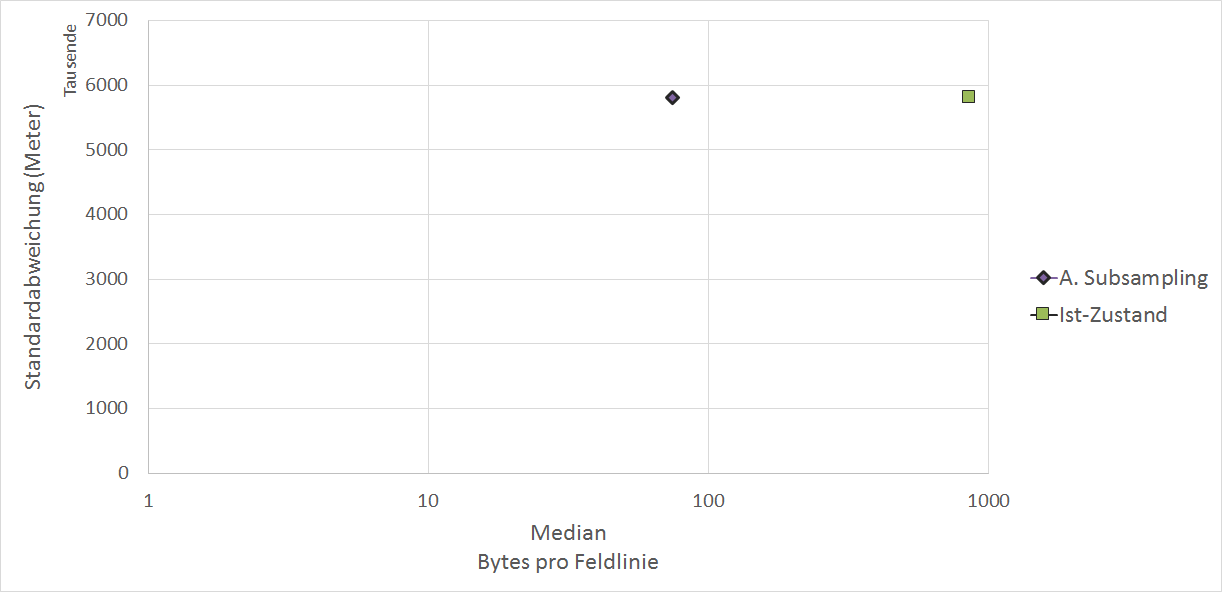
\includegraphics[width=0.8\textwidth,height=6cm,keepaspectratio]{./pictures/resultate/loesung0/loesung0_0.png}
	\caption{Vergleich des Lösungsansatzes: Adaptives Subsampling zur Ist-Kompression.}
	\label{resultate:loesung0:loesung0_0}
\end{figure}
%Grösse der DAtei
Wie im Diagramm \ref{resultate:loesung0:loesung0_0} erkennbar ist, braucht dieser Lösungsansatz deutlich weniger Speicher als die Ist-Kompression. Das Adaptive Subsampling reduziert deutlich die Anzahl Punkte, während die Rar eine bessere Kompression erbringt. Dieser Ansatz kann die Daten um Faktor $11.6$ besser komprimieren.\\
Die Komplexität dieses Ansatzes bleibt ist $O(n)$ ($n$ ist die Anzahl Punkte) und bleibt somit in der selben Komplexitätsklasse wie die Ist-Kompression. Dieser Lösungsansatz ist aber bei der Dekompression schneller, da $n$ etwa vier mal Kleiner ist. und ist som  Da bei der Dekompression $n$ etwa vier Mal weniger Punkte bearbeiten muss, ist die Dekompression sogar schneller als die Ist-Lösung.\\
\begin{figure}[!htbp]
	\center
	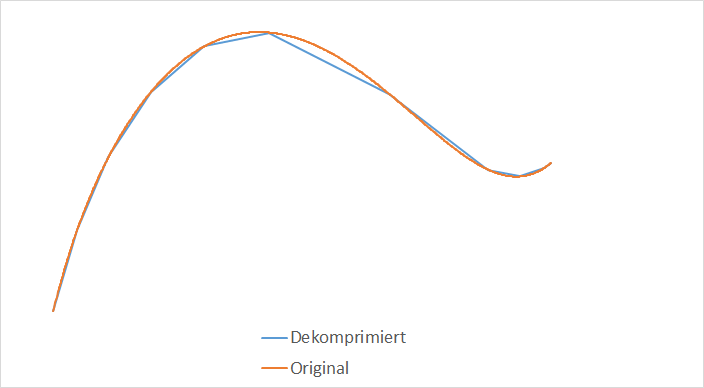
\includegraphics[width=0.8\textwidth,height=6cm,keepaspectratio]{./pictures/resultate/loesung0/loesung0_artefakte.png}
	\caption{Artefakte der Lösung 0}
	\label{resultate:loesung0:artefakte}
\end{figure}
Die Abbildung \ref{resultate:loesung0:artefakte} zeigt die Artefakte, die bei der Komprimierung der Lösung 0 entstehen. Es ist anzumerken, dass der Ist-Zustand die selben Artefakte aufweist.
\pagebreak

\subsection{Lösungansatz: Diskrete Kosinus Transformation}
In diesem Abschnitt wird der Lösungsansatz mittels Diskreter Kosinus Transformation behandelt. Es wurden verschiedene Transformationen getestet, welche eine Approximation mittels Kosinus Funktionen vereinfachen könnten.\\
Um die Feldlinien optimal mit der DCT zu approximieren, müssen "Ringing" Artefakte, welche bei gewissen Feldlinien entstehen, behandelt werden. Diese Artefakte sind für das menschliche Auge störend und begrenzen die Kompressionsrate. Die Artefakte werden im Abschnitt \ref{resultate:loesung1:ringing} besprochen.\\
[\baselineskip]
Für alle Tests wurde eine lineare Quantisierung verwendet. Jeder DCT Koeffizient wird durch einen Faktor geteilt, der sich stetig ehöht. Zum Beispiel wird der erste Koeffizient durch zwei geteilt, der zweite durch Vier, der Dritte durch Sechse etc.  Die Kompressionsrate kann durch einen höheren oder tieferen Faktor gesteuert werden. Diese Quantifizierung ist nicht das Optimum. Eine bessere Quantifizierung wird für die beste Variante ausgearbeitet. Wie die beste Variante im Detail umgesetzt wurde, wird im Abschnitt \ref{konzept:loesung0:kodierung} behandelt. 

\subsubsection{Variante: DCT}\label{resultate:dct}
Diese Variante verwendet einzig die Diskrete Kosinus Transformation und der linearen Quantisierung.
\begin{figure}[!htbp]
	\center
	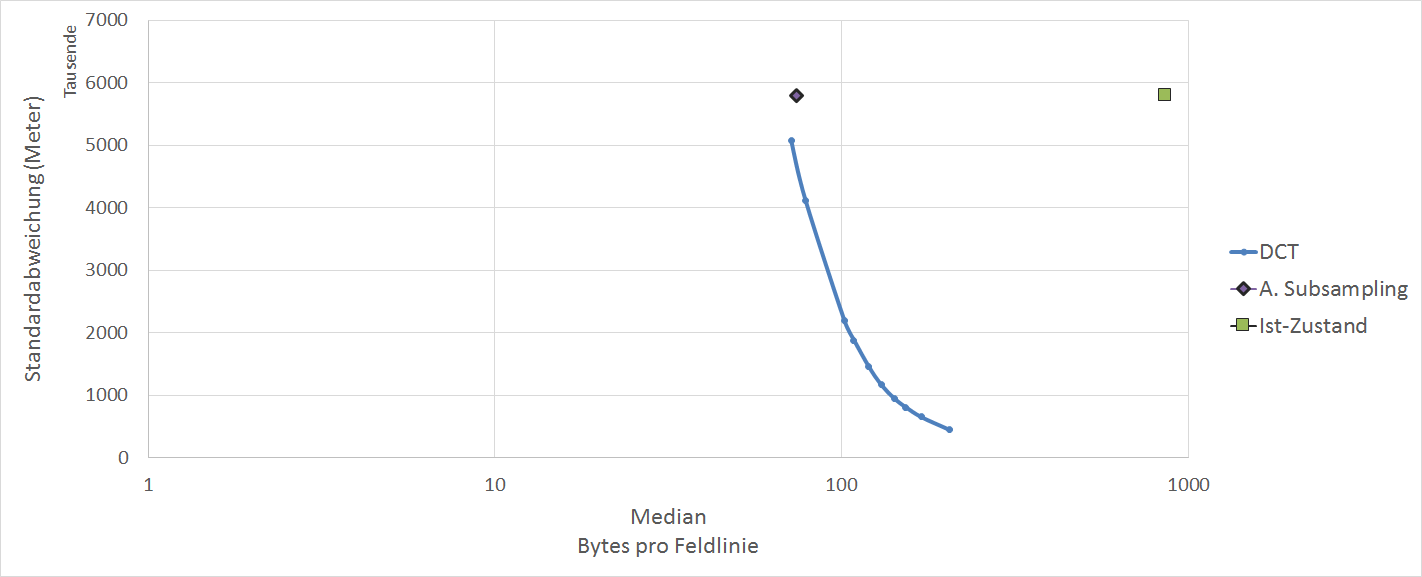
\includegraphics[width=0.8\textwidth,height=6cm,keepaspectratio]{./pictures/resultate/loesung1/loesung1-0/loesung1_0.png}
	\caption{Vergleich der DCT Kompression mit der Lösung0}
	\label{resultate:loesung1:dct:resultate}
\end{figure}
Die Abbildung \ref{resultate:loesung1:dct:resultate} zeigt den Vergleich der DCT Kompression mit dem Lösungsansatz des Adaptiven Subsamplings (siehe \ref{resultate:loesung0}). Es ist deutlich zu erkennen, dass die Standardabweichung schnell steigt bei leicht sinkender Grösse. Der Grund dafür kann im Diagramm der Abbildung \ref{resultate:loesung1:dct:artefakte} entnommen werden. 
\begin{figure}[!htbp]
	\center
	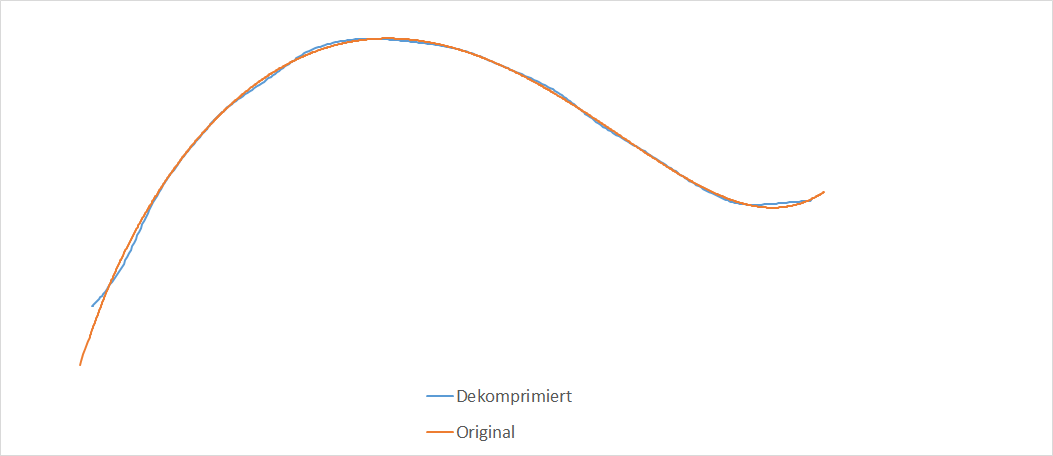
\includegraphics[width=0.8\textwidth,height=6cm,keepaspectratio]{./pictures/resultate/loesung1/loesung1-0/loesung1_0_artefakte.png}
	\caption{Artefakte der DCT Dekompression anhand Beispieldaten}
	\label{resultate:loesung1:dct:artefakte}
\end{figure}
Un den meisten Fällen kann die DCT die Feldlinie gut approximieren. Bei dieser Feldlinie wird der Anfang der Kurve nicht richtig dargestellt. Das ist ein typisches Problem der DCT. Die Diskrete Kosinus Transformation nimmt an, dass das Signal sich periodisch wiederholt. Die implemementierte Transformation (siehe Abschnitt \ref{konzept:loesung1:kosinus}) nimmt an, dass am Anfang und am Ende das Signal in umgekehrter Reihenfolge wiederholt. Bei den Feldlinien kann das zu einer Diskontinuität im Signal führen, welches hochfrequente Kosinus Anteile. Wenn die Quantisierung Hochfrequente Schwingungen verschluckt, entstehen die Artefakte der Abbildung \ref{resultate:loesung1:dct:artefakte}.\\
Eine Möglichkeit ist die Feldlinie um Punkte zu erweitern. Wenn die Feldlinie am Anfang und am Ende abflacht, sollte die resultierende Transformation weniger hochfrequente Schwingungen enthalten. Diese Variante wird im Abschnitt \ref{resultate:loesung1:dct:randbeh+byte} behandelt und führt zu einer deutlich besseren Approximation. Durch eine andere Darstellung der Daten kann das Problem ebenfalls gelöst werden.

\subsubsection{Variante: Ableitung+DCT}\label{resultate:dct:ableitung_dct}
Vor der DCT werden die Feldlinien abgeleitet. Mit der Ableitung soll das Randproblem dargestellt in \ref{resultate:loesung1:dct:artefakte} gelöst werden. Der Nachteil ist, dass Ungenauigkeiten sich durch die Kurve durchziehen und summieren. Am Ende kann die Approximation ungenauer sen, wie am Anfang der Feldlinie.\\
\begin{figure}[!htbp]
	\center
	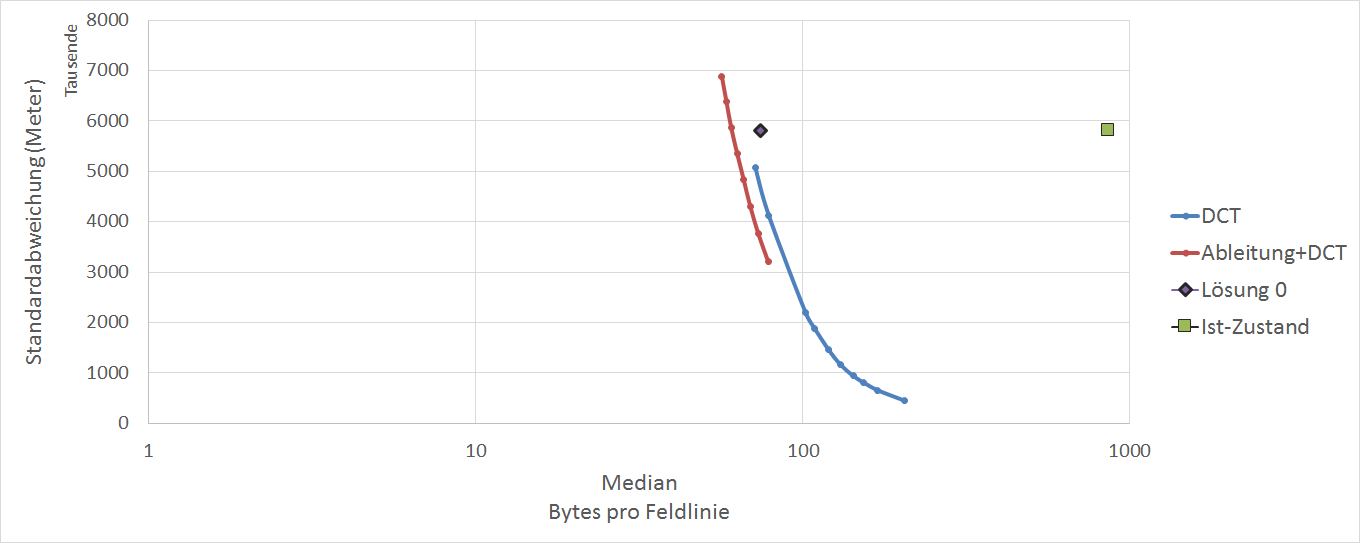
\includegraphics[width=0.8\textwidth,height=6cm,keepaspectratio]{./pictures/resultate/loesung1/loesung1-1/loesung1_1.png}
	\caption{Vergleich der DCT Kompression der Ableitung mit der DCT Kompression}
	\label{resultate:loesung1:dct:artefakte}
\end{figure}
Die abgeleiteten Feldlinien können besser approximiert werden und erreichen dadurch eine Kompressionsrate von $14.3$ mit einer vergleichbaren Genauigkeit. Das Randproblem wurde ebenfalls verbessert. Eine Darstellung der Artefakte ist im Diagramm der Abbildung\ref{resultate:loesung1:dct:byte:artefakte} zu finden.\\
\begin{figure}[!htbp]
	\center
	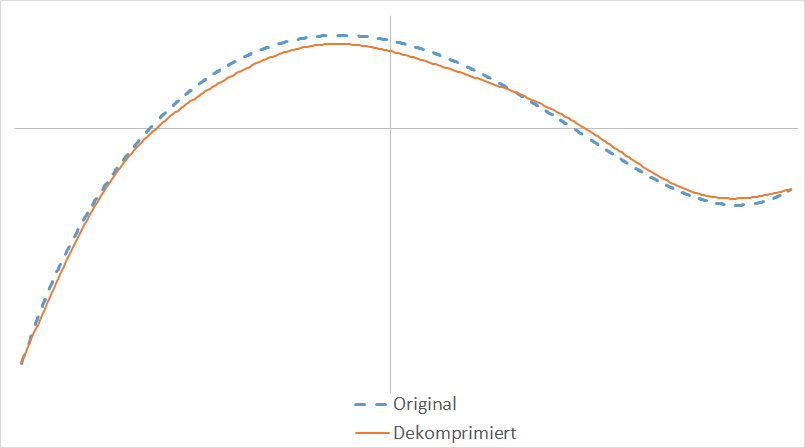
\includegraphics[width=0.8\textwidth,height=6cm,keepaspectratio]{./pictures/resultate/loesung1/loesung1-6/artefakte.png}
	\caption{Artefakte der DCT Kompression der Ableitung}
	\label{resultate:loesung1:dct:byte:artefakte}
\end{figure} 
Es ist deutlich zu sehen, dass die Kurve durch die Quantisierung gedämpft wird. das Maximum der Kurve ist tiefer, sowie das lokale Minima der letzten Halbwelle höher. Der Vorteil dieser Variante ist, dass die resultierende Feldline sehr glatt verläuft. Ohne die Originalkurve währen die Artefakte nicht zu identifizieren.

\subsubsection{Variante: PCA+Ableitung+DCT}
Die Feldlinien liegen meist auf einer Ebene im dreidimensionalen Raum. Wenn die X,Y und Z Kanäle Kosinus-Transformiert werden, ist die Information etwa gleichmässig auf den Kanälen verteilt. Eine Linie könnte sich durch weniger Kosinus-Funktionen approximieren lassen, wenn die Linie zuerst in ein lokales Koordinatensystem transformiert wird.\\
Die Principal Component Analysis (PCA)\cite{abdi2010principal} ist ein Verfahren aus der Statistik, welches Daten in ein neues koordinatensystem Transformiert. Dabei werden die Achsen so gelegt, dass die Daten entlang der ersten Achse die grösste Varianz aufweisen. Entlang der zweiten Achse, welche orthogonal zur ersten liegt, die zweithöchste Varianz etc. Wenn das Vefahren auf die Feldlinien angewandt wird, werden die Feldlinien in ein lokales System transformiert indem der Z-Kanal 0 ist, wenn die Feldlinie in einer Ebene liegt. Der Nachteil ist, dass für die Rücktransformation pro Feldlinie die Koordinatenachsen und die Koordinatenverschiebung abgespeichert werden.\\
Um die PCA wieder rückgängig zu machen, müssen pro Feldlinie sechs Parameter für die neuen Koordinatenachsen und 3 Parameter für die Verschiebung abgespeichert werden. Die Koordinatenachsen werden mit 16 Bit Genauigkeit gespeichert. Die Verschiebung wird Entweder mit 16 oder mit 32 Bit Genauigkeit abgelegt. Die Resultate der 16 und 32 Bit Varianten sind im Diagramm der Abbildung \ref{resultate:loesung1:dct:pca} dargestellt.
\begin{figure}[!htbp]
	\center
	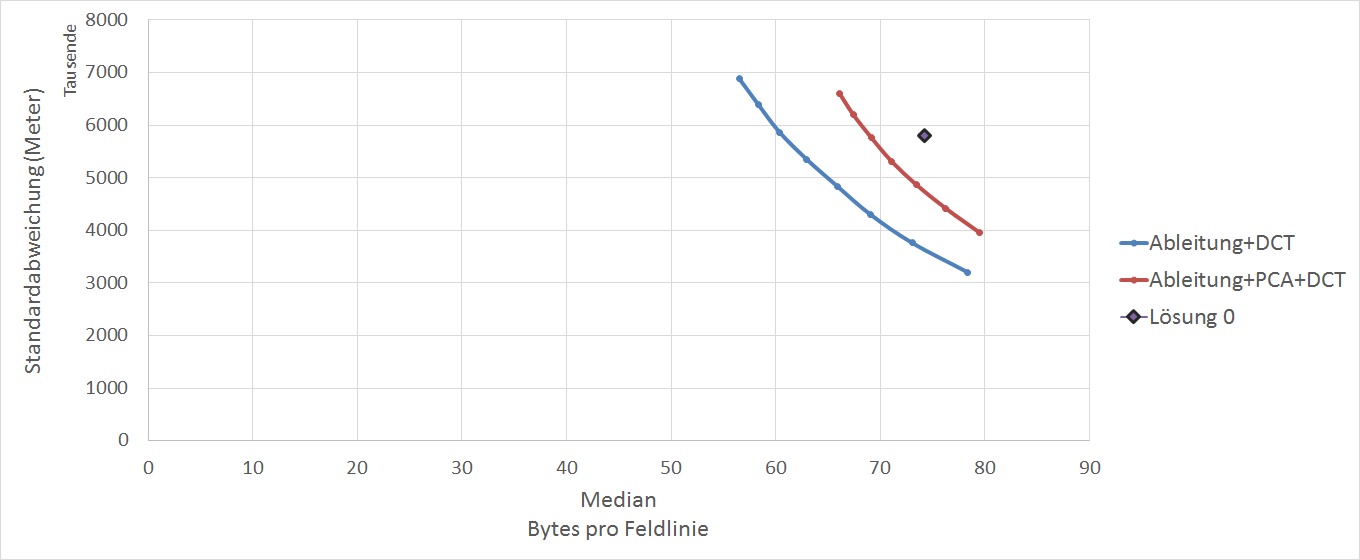
\includegraphics[width=0.8\textwidth,height=6cm,keepaspectratio]{./pictures/resultate/loesung1/loesung1-4/loesung1_4.png}
	\caption{Vergleich der PCA DCT Kompression der Ableitung mit der DCT Kompression der Ableitung}
	\label{resultate:loesung1:dct:pca}
\end{figure}
Beide PCA Varianten erbringen keine bessere Kompression als die Variante ohne PCA (Abschnitt  \ref{resultate:dct:ableitung_dct}). Der Grund ist, dass die Variante ohne PCA zwischen 5 und 20 Kosinus-Funktionen braucht, um eine Feldlinie zu approximieren. Durch die PCA braucht es weniger Funktionen für eine ähnlich gute Approximation. Die zusätzlichen PCA Parameter verbrauchen aber mehr speicherplatz, als die Transformation gewinnt.\\
Interessant ist, dass man mit 16 Bit Genauigkeit keine bessere Approximation erhält. Durch zusätzliche Operationen werden zusätzliche Ungenauigkeiten eingeführt. Es ist als schwer, eine Bessere Kompression mit ähnlicher Genauigkeit zu erhalten, wenn noch mehr transformationen angefügt werden.

\subsubsection{Variante: Ableitung+DCT+Byte Kodierung} \label{resultate:loesung1:ableitung_dct_kodierung}
Eine Feldlinie kann mit 5 bis 20 Kosinusfunktionen approximiert werden. Mit einer besseren Kodierung soll speicherplatz gespart werden. Die Kodierung ist im Abschnitt \ref{konzept:loesung1:kodierung} beschrieben.
\begin{figure}[!htbp]
	\center
	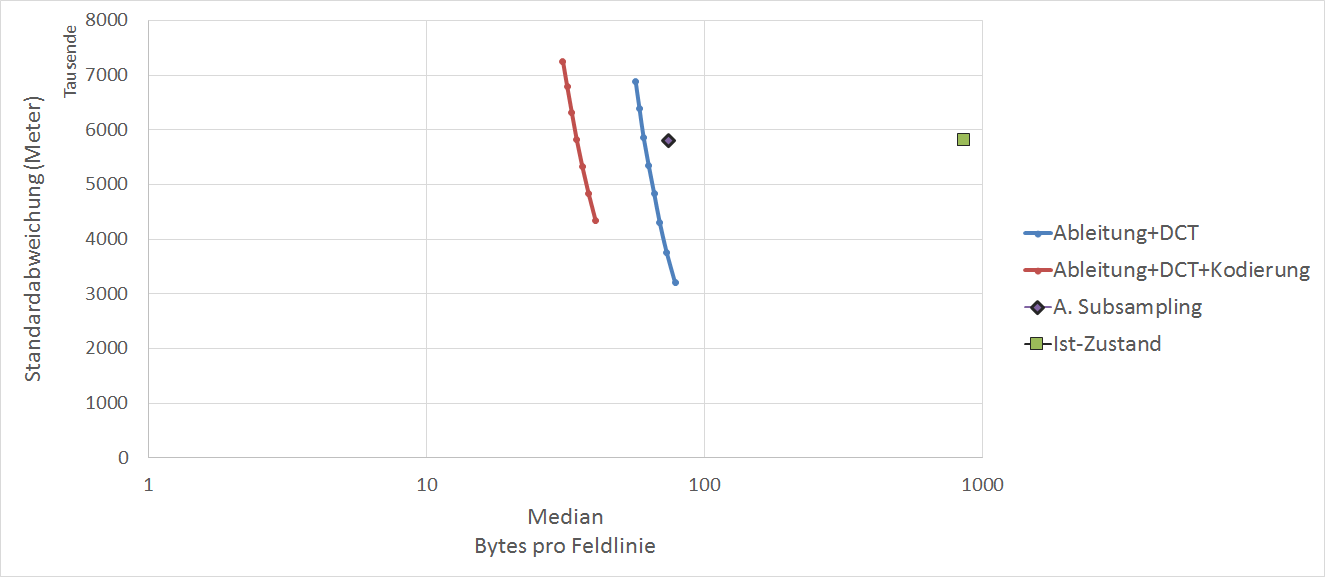
\includegraphics[width=0.8\textwidth,height=6cm,keepaspectratio]{./pictures/resultate/loesung1/loesung1-6/loesung1_6.png}
	\caption{Vergleich der Kompression mit und ohne Byte-Kodierung}
	\label{resultate:loesung1:dct:kodierung}
\end{figure}
Das Diagramm der Abbildung \ref{resultate:loesung1:dct:kodierung} zeigt eine deutliche Verbesserung im Vergleich zum Lösungsansatz "Adaptives Subsampling". Bei einer Vergleichbaren Genauigkeit weist diese Variante eine Kompressionsrate von $24.5$ auf.

\subsubsection{Variante: Randbehandlung+DCT+Byte Kodierung} \label{resultate:loesung1:dct:randbeh+byte}
Wenn  die Artefakte \ref{resultate:loesung1:dct:byte:artefakte} und \ref{resultate:loesung0:artefakte} vergleicht, fällt auf, dass die Variante \ref{resultate:dct} die Feldlinie genauer approximiert. Wenn die Ränder besser dargestellt werden, könnte Variante \ref{resultate:dct} wenigere Kosinus-Funktionen brauchen für eine ähnlich genaue Approximation.\\

Wieder nur die Diskrete Kosinus Transformation, aber noch mit künstlich erzeugten Punkten\ref{konzept:loesung1:randbehandlung} und der Byte Kodierung\ref{konzept:loesung1:kodierung}.
\begin{figure}[!htbp]
	\center
	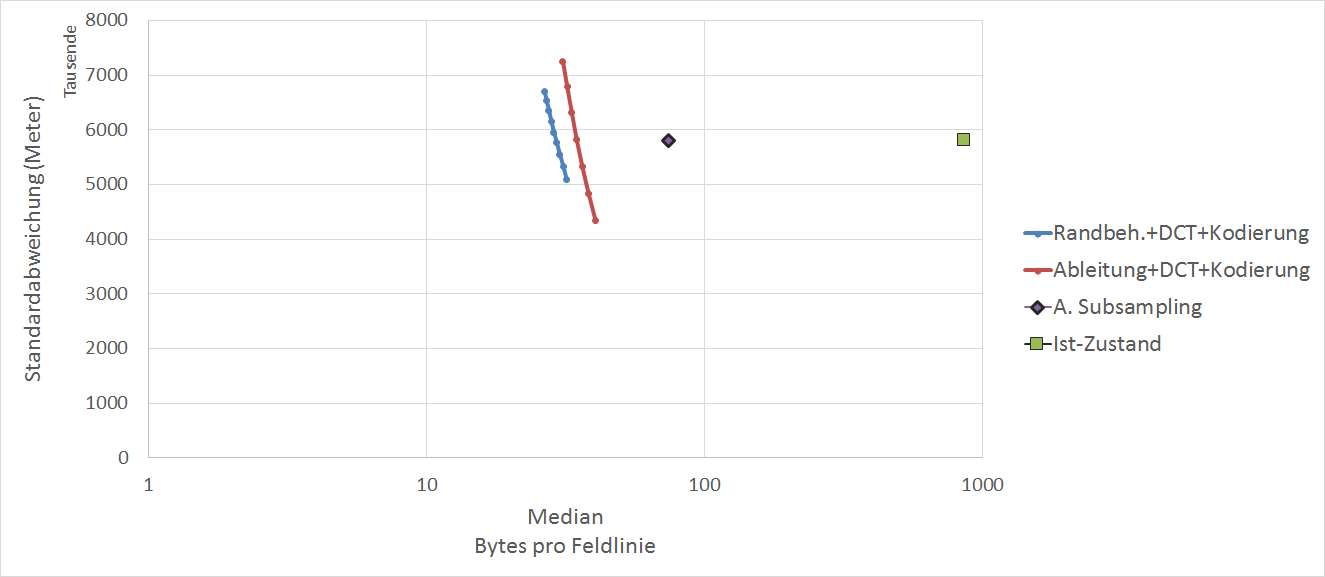
\includegraphics[width=0.8\textwidth,height=6cm,keepaspectratio]{./pictures/resultate/loesung1/loesung1-7/loesung1_7.png}
	\caption{Vergleich der Kompression mit und ohne Byte-Kodierung}
	\label{resultate:loesung1:dct:randbehandlung}
\end{figure}
Das Diagramm der Abbildung \ref{resultate:loesung1:dct:randbehandlung} zeigt den Vergleich der Variante mit Randbehandlung und der Variante der abgeleiteten Feldlinie (beschrieben im Abschnitt \ref{resultate:loesung1:ableitung_dct_kodierung}. Es ist zu erkennen, dass dank der Randbehandlung die Feldlinien mit weniger Bytes ähnlich genau approximiert werden können.

\subsubsection{Ringing Artefakte}\label{resultate:loesung1:ringing}
Obwhol die Variante \ref{resultate:loesung1:dct:randbeh+byte } eine vergleichbare Genauigkeit aufweist, wie Ist-Kompression, sind auf der JHelioviewer visualisierung deutliche Artefakte zu sehen. Die Abbildung \ref{resultate:loesung1:dct:randbehandlung:jvhartefakte} vergleicht die originalen mit dekomprimierten Feldlinien. Die Dekompression Lässt die Feldlinien um das originale Signal schwingen.
\begin{figure}[!htbp]
	\center
	\frame{
	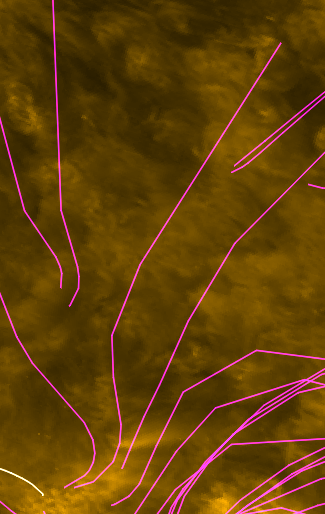
\includegraphics[width=0.8\textwidth,height=6cm,keepaspectratio]{./pictures/resultate/loesung1/loesung1-7/line_good.png}}
		\frame{
	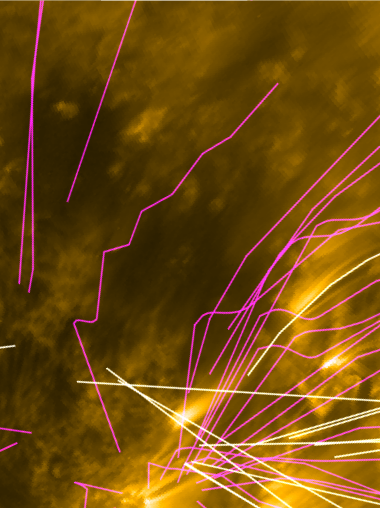
\includegraphics[width=0.8\textwidth,height=6cm,keepaspectratio]{./pictures/resultate/loesung1/loesung1-7/line_bad.png}}
	\caption{Artefakte der Kompression, links sind die originalen Feldlinien, rechts die Dekomprimierten.}
	\label{resultate:loesung1:dct:randbehandlung:jvhartefakte}
\end{figure} 
In diesem Fall scheint die Standardabweichung als Fehlermass zu versagen: Da die Schwingungen nahe am originalen Signal liegen, bleiben die Abstände klein. Jedoch sind die Artefakte für das menschliche Auge inakzeptabel.\\
Interessant ist, dass die die Variante der Ableitung (Abschnitt \ref{resultate:loesung1:ableitung_dct_kodierung}) ähnliche Artefakte aufweist. Im Diagramm der Abbildung \ref{resultate:loesung1:dct:byte:artefakte}, welches die Artefakte anhand einer Beispiellinie zeigt, sind keine Schwinungen zu entdecken. In der JHelioviewer Visualisierung jedoch, sind auch bei dieser Variante deutliche Schwingungen zu erkennen. Die Abbildung \ref{resultate:loesung1:dct:randbehandlung:jvhartefakte_loesung6} zeigt die Artefakte. Es ist anzumerken, dass die Artefakte weniger ausgeprägt sind, aber dennoch störend für das menschliche Auge.\\
\begin{figure}[!htbp]
	\center
	\frame{
	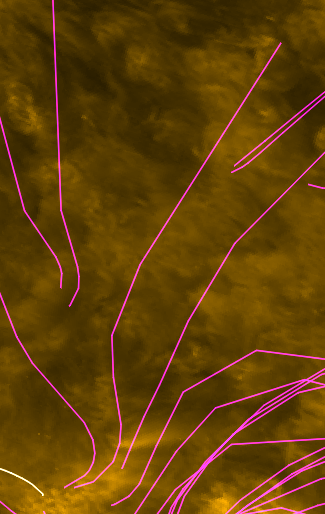
\includegraphics[width=0.8\textwidth,height=6cm,keepaspectratio]{./pictures/resultate/loesung1/loesung1-7/line_good.png}}
		\frame{
	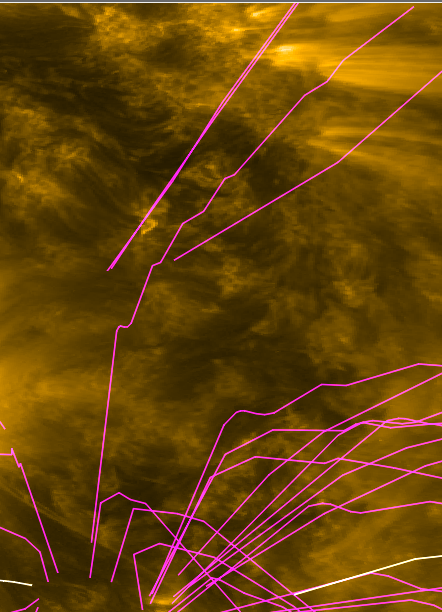
\includegraphics[width=0.8\textwidth,height=6cm,keepaspectratio]{./pictures/testsetup/newalgo//solution6_bad.png}}
	\caption{Artefakte der Kompression, links sind die originalen Feldlinien, rechts die Dekomprimierten der Variante \ref{resultate:loesung1:ableitung_dct_kodierung}.}
	\label{resultate:loesung1:dct:randbehandlung:jvhartefakte_loesung6}
\end{figure} 
Es wird vermutet, dass es sich um Ringing Artifacts \cite{wiki:ringing:artefacts} handelt. 
Sie geschehen, wenn oft bei harten Übergängen in eines Inputsignal und führen zu einem oszillierenden Outputsignal. Ringing Artifacts sind typische Kompressionsartefakte von DCT-basierten Verfahren wie JPEG/JFIF oder MP3.\\
Die Feldlinien, welche am Stärksten von den Artefakten betroffen sind sind die, welche vom Weltall zur Sonne oder von der Sonne ins Weltall führen. Diese verhalten sich oft monoton, mit teils harten Richtungswechsel in der Nähe der Sonnenoberfläche. Die Abbildung \ref{resultate:loesung1:dct:randbehandlung:harte_richtungswechsel} zeigt eine Visualisierung von Feldlinien mit abrupten Richtungswechsel. den abrupten Wechsel gefolgt von einer monotonen Steigung kann nur durch hochfrequente Anteile dargestellt werden. Wenn diese durch die Quantisierung an Genauigkeit verlieren, entstehen die oszillierenden Ringing Artefakte. 
\begin{figure}
	\caption{Harte Richtunswechsel bei Feldlinien, welche von der Sonne zum Weltall führen.}
	\label{resultate:loesung1:dct:randbehandlung:harte_richtungswechsel}
\end{figure}

\subsubsection{Behandlung der Ringing Artefakte}
PCA könnte hilfreich sein, da sich die Artefakte auf einen Kanal beschränken würden. Die einfachste Lösung währe, die Quantisierung herunterzuschrauben.
Resultate der heruntergeschraubten Varianten.